\documentclass[12pt]{article}

\usepackage[margin=25mm,includefoot]{geometry} %includefoot acts on the number of the page

%header und footer zeugs
\usepackage{fancyhdr}
\pagestyle{fancy}
\fancyhead{}%Damit säubern wir den header und footer
\fancyfoot{}
\fancyfoot[R]{\thepage} %Damit machen wir die seitennummer in den footer und mit R schreiben wie sie Rechts

%Graphik Zeugs
\usepackage{graphicx}%Damit kann man photos importieren
\usepackage{float}%damit kann man die positionen von Photos und so ändern (glaube ich)
\usepackage{xfrac}
\usepackage{amsmath}%Fuer Funktionen die ueber Intervalle definiert sind
\usepackage{pdfpages}

\usepackage[hidelinks]{hyperref} %Hyperlinks die aber mit der optiion nicht ins auge fallen

\begin{document}
	\begin{titlepage}
		\begin{center}
		\line(1,0){400}\\
		\vspace{6mm}
		\huge{\bfseries Vakuum}\\
		\vspace{3mm}
		\line(1,0){400}\\
		\textsc{\LARGE Anfängerpraktikum für B.Sc. Physik}\\	
		\textsc{\large Teil II}
		\vspace{10cm}
		\end{center}
		\begin{flushright}
			\textsc{\large Ajello Patrick}\\
			Matr. 03731453\\
			\textsc{\large Luis Walther}\\
			Matr. 03728424\\
			\vspace{2mm}
			21.01.2021
		\end{flushright}
	\end{titlepage}
	
	\tableofcontents
	\thispagestyle{empty}
	\cleardoublepage
	
	\setcounter{page}{1}
	%Wir benutzen label damit wir es später referentieren können
	\section{Abstract}\label{sec:abs} 
	\section{Grundlagen}\label{sec:gru}
	In diesem Versuch werden wir verschiedene Vakuums Techniken benutzen um die Eigenschaften von Idealen Gasen zu untersuchen.Wichtig ist dabei dass Luft sich, bei den gegebenen Drücken wie ein ideales Gas verhält. Das konzept von Vakuum muss auch klar sein: ein echtes Vakuum wäre ein komplett leerer Raum, was nicht realisierbar ist, aber annährbar.
	\subsection{Eigenschaften eines idealen Gaases}
	Ideale Gase folgen der sogenannten \textit{idealen Gasgleichung}:
	\begin{equation} \label{eq: ideale gasgleichung}
	p\cdot V=n \cdot R \cdot T= N \cdot k_B \cdot T
	\end{equation}
	mit p[Pa] der Druck, V[m$^3$] dem Volumen, n[mol] der Anzahl an Mol, R $\approx 8,312 \sfrac {J}{ mol K}$ der Universellen Gaskonstante, T[K] der Temperatur, N der Teilchenzahl und $k_B \approx 1,381 \cdot 10^{-23} \sfrac{J}{K}$ der Boltzmann-Konstante. Eine mol eines Stoffes enthält eine Anzahl an teilchen gleich der Avogadro-Konstante $N_A$. Es gilt der Zusammenhang $R=N_A \cdot k_B$
	\subsubsection{Grundgleichung der Kinetischen Gastheorie}
	Auf Molekularer Ebene fliegen alle Teilche in einem Gas mit verschiedenen geschwindigkeit umher. Zur vereinfachung wird der mittlere Wert $\bar{v}=\sqrt{\bar{v^2}}$ benutzt. Man kann zeigen dass auf die Wände der folgende Druck wirkt
	\begin{equation}
	p= \frac{1}{3}\rho \cdot m \cdot \bar{v^2}
	\end{equation}
	Zusammen mit Gleichung \ref{eq: ideale gasgleichung} ergibt sich
	\begin{equation}
		E_{kin}=\frac{1}{2}m \cdot \bar{v^2} = \frac{3}{2}k_B \cdot T
	\end{equation}
	Im Mittel gilt also eine Proportionalitäts zwischen Kinetischer Energie und Temperatur eines Moleküls.
	\subsubsection{Mittlere freie Weglänge}
	Gasmoleküle kollidieren nicht nur mit den Wänden ihres behälters, sonder auch mit anderen Teilchen. Mit \textit{Mittlerer freier Weglänge($\lambda$)} bezeichnet man die Strecke die die Teilchen im Mittel zurücklegen bevor sie Kollidieren.
	\begin{equation}\label{eq: mittlere freie Weglänge}
		\lambda= \frac{1}{\sqrt{32}\rho F}
	\end{equation}
	mit F den Querschnitt eines Moleküls und $\rho$ die Teilchendichte.
	\subsubsection{Wärmeleitung }
	Der Wärmestrom zwischen zwei Platten ist proportional zum Temperaturunterschied $\Delta T$ und zur Wärmeleitungskonstante $\kappa$ des Gases
	\begin{equation}
	P \propto \kappa \cdot \Delta T
	\end{equation}
	Aus der kinetischen Gastheorie folgt dann für nicht zu kleine Drücke 
	\begin{equation}
		\kappa = \frac{1}{2}\lambda \cdot \rho \cdot k_B \cdot \bar{v}
	\end{equation}
	Mir $\lambda$ aus Gleichung \ref{eq: mittlere freie Weglänge} folgt dann $\lambda\propto \sfrac{1}{\rho} $, d.h $\kappa$ ist unabhängig von der Gasdichte. Bei kleinen Drücken wird $\lambda$ aber gleich oder größer als der Abstand zwischen den Platten und damit folgt dass $\kappa  \propto \rho $. Diese Eigenschaft nutzen wir in diesem Experiment beim Piranimanometer aus.
	\subsubsection{Viskosität eines idealen Gases}
	Für die Viskosität eines idealen Gases gilt
	\begin{equation}
		\nu = \frac{1}{3}\lambda \cdot\rho\cdot m \cdot \bar{v}
	\end{equation}
	Bei Drücken von über 1 hPa wird auch die Viskosität $\nu$ unabhängig von der Dichte. Dann gilt auch $\nu  \propto \rho $
	\subsubsection{Druckmessung}
	Die direkte Methode Druck zu messen ist die Kraft zu messen die auf eine Fläche ausgeübt wird. Dafür kann man zum Beispiel ein Quecksilbermanometer oder ein Membran-Manometer benutzen.
	Andere Arten von Manometer sind Wärmeleitungsmanometer wie das Piranimanometer in diesem Experiment, Kaltkathodenmanometer und Ionisationsmanometer. All diese Instrumente müssen vor der benutzung vor kalibriert werden.
	
	\subsection{Vakuumstechnische Begriffe}
	Eine Vakuumapparatur besteht aus einem Rezipienten der zu evakuieren ist und einer Pumpe. In diesem Versuch wird eine Drehschieberpumpe benutzt die aus 2 Rotoren besteht die durch Schieber und dass sich drehen die abgesaugte Luft raus schieben. Es wird üblicherweise ein Endvakuum von $10^{-3}$hPa und niedriger erreicht. Dieses Vakuum wird als \textit{Feinvakuum} klassifiziert. Am Anfang des Saugvorgangs befinden wir uns noch im \textit{Grobvakuum} (1-1000hPa). Höhere Arten von Vakuum werden nicht erreicht.
	
		\begin{figure}[h]
		\centering
		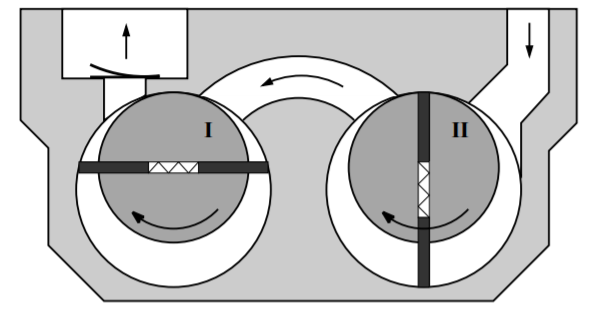
\includegraphics[width=10cm]{Drehschiebepumpe.png}
		\caption{Drehschiebepumpe im Schnitt}
		\label{fig: Drehschiebepumpe}
		\end{figure}
	Die \textit{Saugleistung} einer Pumpe $Q_p=\frac{p\cdot V}{dt}$ ist bei der Drehschiebepumpe über einen Bereich proportional zum Druck.
	\begin{equation}
		Q_p=S \cdot p
	\end{equation}
	S ist das Saugvermögen. Es gilt also
	\begin{equation}\label{eq: Saugen}
		\frac{d(p\cdot V)}{dt}=S \cdot p
	\end{equation}
	Das Saugvermögen kann aber praktisch nie ganz ausgenutzt werden weil es begrenzt wird von den kleinen leitwerten von Rohren, Engstelle, usw. Für das effektive Saugvermögen gilt
	\begin{equation}
		\frac{1}{S_{eff}}=\frac{1}{S}+\frac{1}{L_1}+\frac{1}{L_2}+...
	\end{equation}
	mit $L_{1,2,...}$ die Leitwerte der hintereinander geschalteten Komponenten.
	Seien $S_{eff}$ und V überall konstant dann bekommt man durch Integration der Gleichung \ref{eq: Saugen}.
	\begin{equation}\label{eq: exp sauen}
		p(t)=p_0 \cdot exp(-\frac{S_{eff}}{V}\cdot t)
	\end{equation}
	$S_{eff}$ ist normalerweise auf großen Bereichen nicht konstant aber man kann Gleichung trotzdem auf kleine bereiche anwenden wo $S_{eff}$ annähernd konstant ist.
	\subsection{Gasströmung und Leitwerte}
	Bei hohen Drucken kann  man Gas als zähes Medium sehen und das Hagen-Poiseuillsche Gesetz anwenden. Wenn man statt dem Volumenstrom durch das Rohr den Gasmengenstrom betrachtet erhält man die Formel
	\begin{equation}
		Q= p(x) \cdot \frac{\pi \cdot d^4}{128 \cdot \eta }\cdot \frac{dp}{dx}
	\end{equation}
	mit d Rohrdurchmesser.
	Da die strömende Menge des Gases im ganzen Rohr konstant sein muss ist Q unabhängig von x. Daraus folgt $p(x)\cdot \frac{dp}{dx}$ muss konstant sein. Mann kann schreiben
	\begin{equation}
		Q=\frac{\pi \cdot d^4}{128 \cdot \eta \cdot l }\cdot \bar{p}\cdot \Delta p = L\cdot \Delta p
	\end{equation}
	mit L dem Leitwert des Rohrs
	\begin{equation}\label{eq: leitwert}
		L=\frac{\pi \cdot d^4}{128 \cdot \eta \cdot l }\cdot \bar{p}
	\end{equation}
	Bei niedringen Drücken wird die Gleichung \ref{eq: leitwert} ungültig und wenn man $\lambda$ mit dem Rohrdurchmesser ersetzt erhält man
	\begin{equation}
		L=\sqrt{\frac{\pi \cdot k_B \cdot T}{18 \cdot m}}\cdot \frac{d^3}{l}
	\end{equation}
	In unseren Laborbedingungen bei $20\textdegree C$ gilt dann
	\begin{equation}\label{eq: mol strom}
		L= 121 \frac{m}{s}\cdot \frac{d^3}{l}
	\end{equation}

	Im dritten Teil unseres Experimentes haben wir einen Aufbau mit einer Reihenschaltung  von Rohren, dort gilt 
	\begin{equation}\label{eq: eff saugen}
		\frac{1}{L_{gesamt}}=\frac{1}{L_1}+\frac{1}{L_2}+...
	\end{equation}	
	\subsection{Pirani-Manometer}
	In der Messröhre befindet sich ein dünner Draht (in unserem Versuch Wolframdraht mit $10 \mu m$ durchmesser). Seine Temperatur und damit sein Widerstand wird konstant gehalten. Die Leistung die dafür gebraucht wird ist dann proportional zur Wärmeleitfähigkeit des Gases. gemessen wird der Strom I.
	
	  
	\section{Experimentelles Vorgehen}\label{sec:exp}
	\subsection{Kalibrierung des Pirani-Manometers}
 
		\begin{figure}[H]
		\centering
		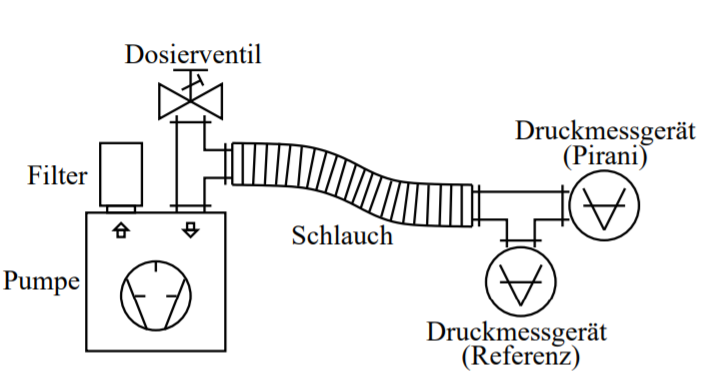
\includegraphics[width=10 cm]{kalibrierung.png}
		\caption{Aufbau zur kalibrierung des Pirani-Manometers}
		\label{fig: kalibrierung}
		\end{figure}
		Nach dem Aufbau des Versuchs wie im folgenden Bild, den wert des Stroms bei mindestens 20 verschiedenen Drücken messen. Die Pumpe einschalten bis man auf einen konstanten druck kommt. Bei kleinen Drücken wird dies nur erreicht wenn man die Pumpe anlässt. Bei höheren Drücken die Pumpe zwischen Messungen ausmachen. Durch das Dosierventil kann Luft rausgelassen werden.
	\subsection{Saugvermögen der Pumpe}
	Man schließt die Pumpe wie in der folgenden Figur an einen Kolben an und misst die Zeit die gebraucht wird um 80ml Volumen auszusaugen. Der Dreiwegehahn ermöglicht es uns Messungen zu haben die nicht von dem Einschaltungsprozess der Pumpe und der Luft die im Schlauch zwischen pumpe und Kolben ist, verfälscht sind. Der Hahn wird erstmal zu gehalten, dies ermöglicht der Pumpe einen konstanten druck im Hahn zu kreieren, der dann, wenn man den dreiwegehahn dreht an dem Kolben zieht.
	\begin{figure}[H]
		\centering
		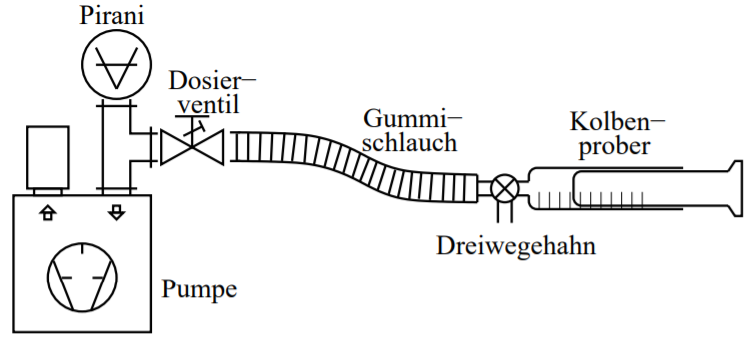
\includegraphics[width=10cm]{Saugvermoegen.png}
		\label{fig: Saugvermögen }
		\caption{Aufbau zur messung des Sehvermögens der Pumpe}
	\end{figure}
	\subsection{Effektives Saugvermögen der Pumpe}
	Ein Mssing- Rezipient wird wie in der Figur mit 3 verschiedenen Verbindungsrohren ausgepumpt. Das Volumen vom Messing Behälter beträgt V= $(3,0\pm 0,1)dm^3$.
	Die verbidungen sind: 
	\begin{itemize}
		\item Schlauch mit 22mm durchmesser über 2 Minuten.
		\item Schlauch mit Kapillare mit $(2,0\pm 0,1)mm$ Durchmesser und $(9,5\pm 0,2)cm$ Länge über 8 Minuten. 
		\item Schlauch mit Kapillare mit $(3,0\pm 0,1)mm$ Durchmesser und $(9,5\pm 0,2)cm$ Länge über 6 Minuten.
	\end{itemize} 
	
	\begin{figure}[H]
		\centering
		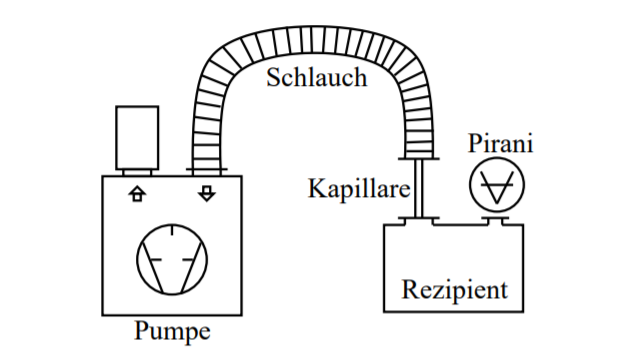
\includegraphics[width=10cm]{Auspumpzeit.png}
		\label{fig: Saugvermögen }
		\caption{Aufbau zur messung effektiven Sehvermögens der Pumpe}
	\end{figure}
	
	\section{Diskussion}\label{sec:dis}
	\subsection{Kalibrierkurve}
	Die Kalibrierkurve kann in verschieden Bereiche geteilt werden, von besonderem Interesse ist der Bereich zwischen 20 und 55 Ampere, da wir dort unsere Messungen für das Saugvermögen durchgefürt haben. Einen ersten Bereich ist der zwischen 17 und 34 A, dort sieht man ein lineare Abhangigheit zwischen Druck und Strom. 
		\begin{figure}[H]
		\centering
		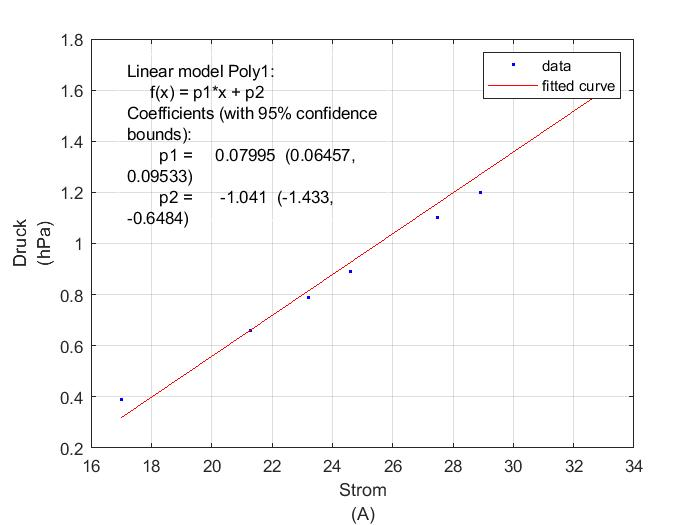
\includegraphics[width=10cm]{Kalibrierung (17-32).jpg}
		\label{fig: Kalibrierung(17-32)}
		\end{figure}
	Wir haben eigentlich noch Messungen die unter diesem Bereich liegen aber wegen der geringen Anzahl (n=2), der nichtlinearität des Anstieg und da sie nicht für die Kalibrierung relevant sind, da unsere Messungen weit entfernt sind, wird dieser Bereich bis auf weiteres ignoriert. 
	
	Ein zweiter Bereich der von interesse ist, ist der zwischen 34 und 72 Ampere, dort ist der Wachstum exponentiell.
			\begin{figure}[H]
				\centering
				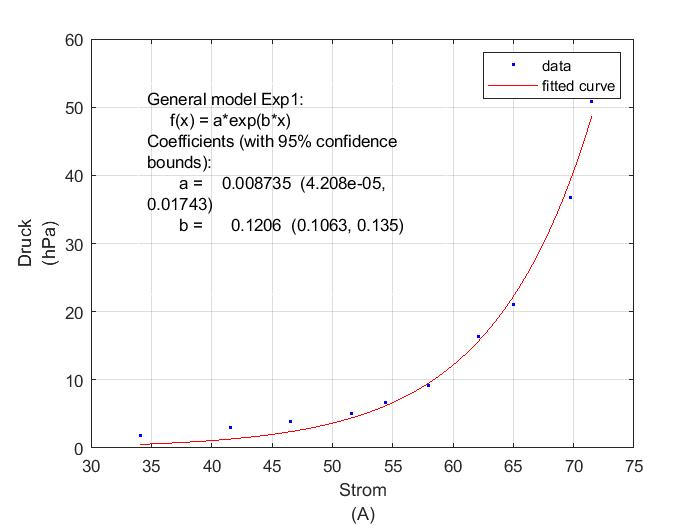
\includegraphics[width=10cm]{Kalibrierung (32-71).jpg}
				\label{fig: Kalibrierung(32-71)}
			\end{figure}
	In dem bereich danach wächst der Druck sehr stark an, fast so als waeren wir nahe an einer Singularitaet.
	
	\begin{figure}
		\centering
		\begin{minipage}{0.45\textwidth}
			\centering
			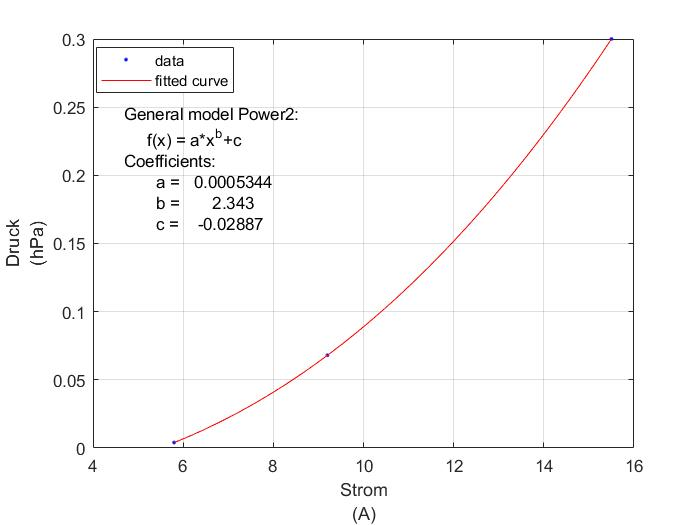
\includegraphics[width=0.9\textwidth]{kalibrierung(0-17).jpg} % first figure itself
			\caption{Kalibrierungskurve I$<$17A. Keine wirkliche statistische relevanz wegen n=3, aber ist für Aufgabe 3 notwendig}
		\end{minipage}\hfill
		\begin{minipage}{0.45\textwidth}
			\centering
			\includegraphics[width=0.9\textwidth]{kalibrierung(71+).jpg} % second figure itself
			\caption{Kalibrierungskurve I$>$74A}
		\end{minipage}
	\end{figure}
	
	Man kennt den zusammenhang zwischen Leistung P und Stromstärke $P=RI^2$ mit den gegeben widerstands $\Omega 44$. Um den Strom auszurechnen stellen wir die zwei Gleichungen die wir durch den Fit gewonnen haben nach I um. Wir erhalten dann
	\begin{equation}
	\begin{cases}
		I(p)=\frac{p+1.041}{0.07995} & 17\leq I \leq 34 \\
		I(p)=\frac{1}{0.1206}\ln\frac{p}{0.008735} & 34\leq I \leq 72\\
	\end{cases}
	\end{equation}
	Die bereiche haben natürlich keine scharfen grenzen wie es hier in den Formeln aussieht. Dass ist aber für dieses experiment von weniger Bedeutung.
	Es ist uns jetzt möglich durch die Fehler von dem Druck die Fehler der Leistung zu berechnen. Es sind vom Hersteller 2 Unsicherheiten angegeben. Für das Grobvakuum ist der Gesamtfehler $\Delta p_{g}=0.08 \cdot p$ . Für das Feinvakuum 20\%p+2Digits und eine Auflösung von A=0.001hPa.
	
		\begin{figure}[H]
		\centering
		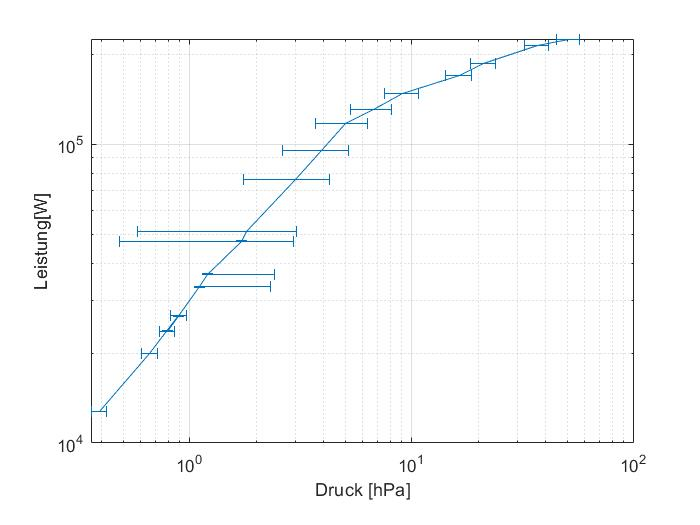
\includegraphics[width=10cm]{Druck-Leistung.jpg}
		\label{fig: Druck-Leistung}
		\caption{Leistung als Funktion vom Druck. Doppellogaritmische Skala}
		\end{figure}
	Im unteren Bereich, bis zum Druck von 1 hPa sieht man aus dem Graphen sofort dass es linear ist. Im Bereich 1-10 hPa findet man immer noch ein wenig von  diesem Verhalten, auch wenn weniger markant, danach ist die linearität nicht mehr vorhanden. De Vermutung ist dass das Verhalte sich zwischen Grob und Feinvakuum verandert und die zone zwischen 1-10 hPa eine Transitionszone ist mit gemischtem verhalten. Die Fehler der Leistung sind extrem klein. Das ist so weil für  größeren Werte von dem Druck als Fit eine exponentialkurve benutzt würde, nach dem strom umgestellt gibt dass eine logarithmische kurve die nach p abgeleitet auf einen $\sfrac{1}{p}$ Term im F ehler führt. Daraus folgt dass der Fehler invers proportional zu p ist. Es kann sein dass gaußsche  Fehlerfortpflanzung in diesem Falle nicht die beste Lösung ist da dass auf so extrem kleine Fehler führt.
	
	\subsection{Saugvermögen der Pumpe}
	Das Saugvermoegen der Pumpe wurde durch die Formel \ref{eq: Saugen} berechnet. $\sfrac{\partial V}{\partial t}$ wird hier zu  $\sfrac{\Delta V}{\Delta t}$ diskretisiert. Wir erhalten so de folgende Formel
	\begin{equation}
		S= \frac{V \cdot p_0}{t\cdot p}
	\end{equation}
	mit $p_0=960mbar$ dem Normaldruck in Garching. 
	In 
	\begin{table} [H]
		\begin{center}
			\caption{Ergbnisse bei konstantem Strom}
			\begin{tabular}{l|c|r}
				\textbf{p[hPa]} & \textbf{$\Delta t [s]$}  & \textbf{S $[\sfrac{m^3}{h}]$}\\
				\hline
				0,6699$\pm{0,1040}$ & 247,7333$\pm{1,0000}$ & 1,2470$\pm{0,5436}$\\
				1,2536$\pm{1,2117}$ & 112,1133$\pm{0,5000}$ & 1,6919$\pm{0,4639}$\\
				1,3671$\pm{1,2103}$ & 49,8200$\pm{0,2500}$  & 6,5447$\pm{1,4884}$\\
				4,6779$\pm{1,3160}$ & 35,5967$\pm{0,2500}$  & 4,6175$\pm{0,3582}$\\
			\end{tabular}
		\end{center}
	\end{table}

	In der folgenden tabelle sehen wir den zusammenhang zwischen vier verschiedenen Drücken und dem Saugvermögen. Gemittelt erhalten wir als Saugvermögen $(3,5253\pm 0,7135)\sfrac{m^3}{h}$, was im Mittel recht gut mit der Herstellerangabe von $3,7\sfrac{m^3}{h}$ übereinstimmt.
	Man muss aber feststellen dass alle einzelnen errechneten Werte von S recht weit entfernt davon sind und mit nur 4 Messunge es schwer is zu behaupten dass sich statische Fehler untereinander aufgehoben haben. Diese ungenauigkeit kann an der großen unsicherheit der Pirani-manometers bei geringen Drücken liegen.
	
	\subsection{Effektives Saugvermögen der Pumpe}
	\begin{figure}[H]
		\centering
		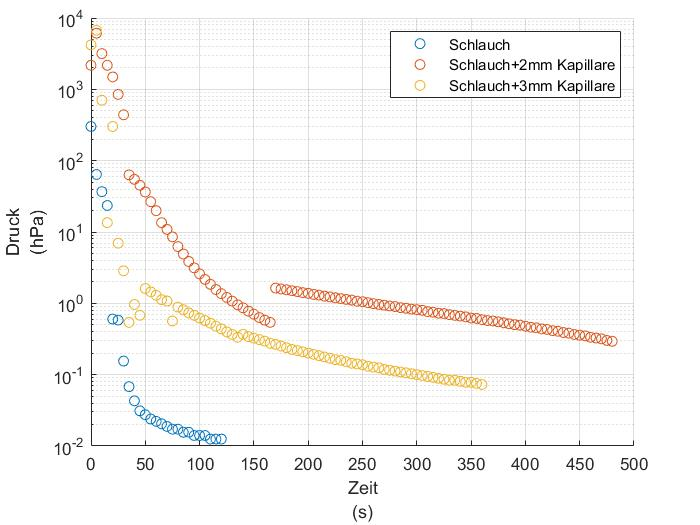
\includegraphics[width=10cm]{Druck-Pumpzeit.jpg}
		\label{fig: Zeit-Druck}
		\caption{Druck als Funktion der Zeit für die drei verschiedenen Verbindungen. Halblogaritmische Skala}
	\end{figure}
	Besonders markant sind die Stellen im Graphen wo der Druck springt. Dies ist kein physikalisches Phenomen, sonder liegt daran dass an diesen punkte die funktion die zum fitten benutzt wurde sich ändert und dort nicht zuverlässig ist. 
	Man sieht auch sofort die hohen Anfangs Drücke; bei allen Messungen ist der Druck kurz nach oben geschossen, bevor er angefangen hat schnell zu fallen. Dies liegt wahrscheinlich am Instrument da es keinen Grund gibt warum im gefäß der Druck höher sein sollte als außen, wenn wie keine Luft reingepumpt haben.
	Das effektive Saugvermögen lässt sich durch Gleichung \ref{eq: exp sauen} bestimmen.
	\begin{equation}
		S_{eff}=- \ln \left(\frac{p(t)}{p_0}  \right)\cdot \left( \frac{V}{t}\right)
	\end{equation} 
	Der theoretische Wert wird bestimmt durch die Gleichung \ref{eq: eff saugen}. Mit $S=3,7\frac{m^3}{h}$, und L durch Gleichung \ref{eq: leitwert} für viskose Strömung 
	und \ref{eq: mol strom} für molekulare Strömung. $\eta_{luft}$ sei gegeben als $1,82 \cdot 10^{-5}\sfrac{kg}{ms}$ und $\bar{p}$ sei gegeben als 5hPa.
	Die logaritmische Steigung ist gegeben durch
	\begin{equation}
			m_{eff}=\frac{ln(p)-ln(p_0)}{t}
	\end{equation}
		\begin{table} [H]
		\begin{center}
			\caption{Logaritmische Steigung}
			\begin{tabular}{l|c|c|r}
				\textbf{Strömung } & \textbf{Schlauch}  & \textbf{Kapillare 3mm} & \textbf{Kapillare 2mm}\\
				\hline
					Viskos    &	-0,54175     & -0,72713 & -0,90309\\
					Molekular & 	-0,85256 & -1,44283 & -1,09469\\
			\end{tabular}
		\end{center}
		\end{table}
		\begin{table} [H]
			\begin{center}
				\caption{Theoretische Leeitwerte $\sfrac{m^3}{h}$}
				\begin{tabular}{l|c|c|r}
					\textbf{Strömung } & \textbf{Schlauch}  & \textbf{Kapillare 3mm} & \textbf{Kapillare 2mm}\\
					\hline
					Viskos    &	$(1,50\pm 0.02)\cdot 10^{3} $    & $ (2,1\pm 0,3 )$ & $ (0,41\pm 0.01 )$\\
					Molekular & $ (10,8\pm1,1 )$ & $ (0,13\pm 1,01 )$ & $ (37\pm 5 )\cdot 10^{-3}$\\
				\end{tabular}
			\end{center}
		\end{table}
	Für die theoretischen Leitwerte wurden Formeln \ref{eq: mol strom} und \ref{eq: leitwert} benutzt.
	
		\begin{table} [H]
			\begin{center}
				\caption{Theoretisches effektive Saugvermögen $\sfrac{m^3}{h}$ }
				\begin{tabular}{l|c|c|r}
					\textbf{Strömung } & \textbf{Schlauch}  & \textbf{Kapillare 3mm} & \textbf{Kapillare 2mm}\\
					\hline
					Viskos    &	$( 3,69\pm 0,01)$ & $(1,3 \pm 0,2 )$ & $( 0,37\pm 0,06)$\\
					Molekular &	$( 2,7\pm 0,1 )$ & $(0,12 \pm 0,01 )$ & $( 0,035\pm 0,005)$\\
				\end{tabular}
			\end{center}
		\end{table}
		\begin{table} [H]
			\begin{center}
				\caption{Experimentelles effektive Saugvermögen $\sfrac{m^3}{h}$ }
				\begin{tabular}{l|c|r}
					\textbf{Strömung } & \textbf{Schlauch}  & \textbf{Kapillare 3mm} \\
					\hline
					Viskos    &	$( 4,0133 \pm 0,0701)$ & $( 0,7992\pm 0,0259 )$ \\
					Molekular &	$( 1,9401 \pm 0,0014)$ & $( 3,4360\pm 0,0014)$ \\
				\end{tabular}
			\end{center}
		\end{table}
	Drei von Vier Werten liegen in der Selben größenordnung, auch wenn sie im Fehler nicht übereinstimmen, weil die Fehler extrem klein sind gegen unsere Daten. Nur der Wert für Molekulare strömung bei der 3mm Kapillaren ist sehr anders als der theoretisch errechnete. Eine sehr große Fehlerquelle die aber nicht direkt im Fehler quantifiziert wurde ist die Ungenauigkeit des Fits über große Bereiche, besonders markant in der Figur \ref{fig: Zeit-Druck}, wo die “Funktion” sogar unstetig ist, für dass es in diesem experiment keinen physikalischen Grund gibt.
	
	
 	\subsection{Fragen}
 	\subsubsection{Frage 1}
 	Viskose Strömung entsteht bei Grobvakuum, wo es noch, im vergleich mit Fein und Hochvakuum, viele Moleküle gibt. Dies bedeutet dass die mittlere freie Weglänge sehr kurz ist und es viele Kollisionen zwischen Molekülen gibt. Für Molekulare Strömung ist ein stärkeres Vakuum nötig. Da die Teilchendichte dort geringer ist gibt es auch weniger Kollisionen und die mittlere freier Weglänge ist größer.
 	
 	\subsubsection{Frage 2}
 	Durch Vergleich mit Abbildung \ref{fig: Zeit-Druck} und der Annahme dass sich das benehmen des Drucks bei einem Kapillar von d=1mm nicht von den anderen verändert, kann man vermuten dass der Druck nach 10 Minuten etwas über 1 hPa sein wird.
 	\subsubsection{Frage 3}
 	Mit der Gleichung \ref{eq: ideale gasgleichung} kann man den Druck bei 1 Molekül pro $m^3$
 	\begin{equation}
		p=\frac{N}{V}\cdot k_b \cdot T \approx4,04 \cdot 10^{-21}Pa
 	\end{equation}
 	angenommen Tempeatur=20\textdegree C
	\section{Anhang}\label{sec:anh}
	\subsection{Fehlerechnung}
	\subsubsection{kalibrierkurve}
	Für die Leistung des Manometers haben wir die Fehler wie folgt berechnet:
	\begin{equation}
		\Delta P= \sqrt{(\Delta R)^2+ \left(\frac{\partial P}{\partial I}\right)^2\cdot (\Delta I)^2}
	\end{equation}
	mit $\Delta I = \left(\frac{\partial I}{\partial p}\right)\cdot \Delta p $ unterteilt wie folgt
	\begin{equation*}
	\begin{cases}
		\left(\frac{\partial I}{\partial p}\right)= \frac{1}{0.0795} &  0.39 \leq p \leq 0.79 \\
		\left(\frac{\partial I}{\partial p}\right)= \frac{1}{0.0795} & 1.1 \leq p \leq 1.7 \\
		\left(\frac{\partial I}{\partial p}\right)= \frac{1}{0.1206 \cdot p} & 1.7 \leq p \leq 72 \\
	\end{cases}
	\begin{cases}
		\Delta p_{Grob}= 0.08 \cdot p  &  0.39 \leq p \leq 0.79 \\
		\Delta p_{Fein}=\sqrt{\left(\frac{\frac{20}{100}\cdot p}{\sqrt{3}}\right)^2+(2Digits+1)^2+\left(\frac{0.001}{\sqrt{3}}\right)^2} & 1.1 \leq p \leq 1.7 \\
		\Delta p_{Fein}=\sqrt{\left(\frac{\frac{20}{100}\cdot p}{\sqrt{3}}\right)^2+(2Digits+1)^2+\left(\frac{0.001}{\sqrt{3}}\right)^2} & 1.7 \leq p \leq 72 \\
	\end{cases}
	\end{equation*}
	\subsubsection{Saugvermögen der Pumpe} 
	 \begin{equation}
		S= \frac{dV}{dt}\cdot \frac{p_0}{p}
	\end{equation}
	\begin{equation}	
		\Delta S= \sqrt{\left(\frac{\partial S}{\partial V}\cdot \Delta V\right)^2+\left(\frac{\partial S}{\partial t}\cdot\Delta t \right)^2+\left(\frac{\partial S}{\partial p}\cdot\Delta p \right)^2}
	 \end{equation}
 \begin{equation}
 	\Delta p = \sqrt{(\Delta p_{Grob/fein*})^2+\left(\frac{\partial p}{\partial I}\cdot \Delta I\right)^2}
 \end{equation}
 mit $\Delta p_{grob}$ und $\Delta p_{fein}$ aus der vorherigen Aufgabe.
\subsubsection{Effektives Saugvermögen der Pumpe}
Im viskosen Bereich gilt Gleichung \ref{eq: leitwert}, im molekularem \ref{eq: mol strom}.. Der Fehler bleibt:
\begin{equation}
	\Delta L=\sqrt{\left(\frac{\partial L}{\partial d}\cdot \Delta d\right)^2+\left(\frac{\partial L}{\partial l}\cdot \Delta l\right)^2}
\end{equation}
Für die Berechnung des Fehlers des effektiven Saugvermögen würde Gaußsche Fehlerfortpflanzung benutzt, für die Variablen V, mit gegebenem Fehler, und p, mit Fehler errechnet so wie in den vorherigen aufgaben mit verschiedenen Formeln für viskose und molekulare Strömung
	
\subsection{Literaturverzeichnis}\label{sec:lit}
	\begin{description}
	\item[-]https://www.ph.tum.de/academics/org/labs/ap/ap2/VAK.pdf
	\item[-]Praktikumsseite auf Moodle
	\item[-]Demtröder Experimentalphysik 2, ISBN 978-3-642-29944-5
	\item[-]https://www.ph.tum.de/academics/org/labs/ap/org/ABW.pdf
\end{description}
\subsection{Bilderverzeichnis}
\begin{description}
	\item[-]https://www.ph.tum.de/academics/org/labs/ap/ap2/VAK.pdf
\end{description}
\subsection{Daten}
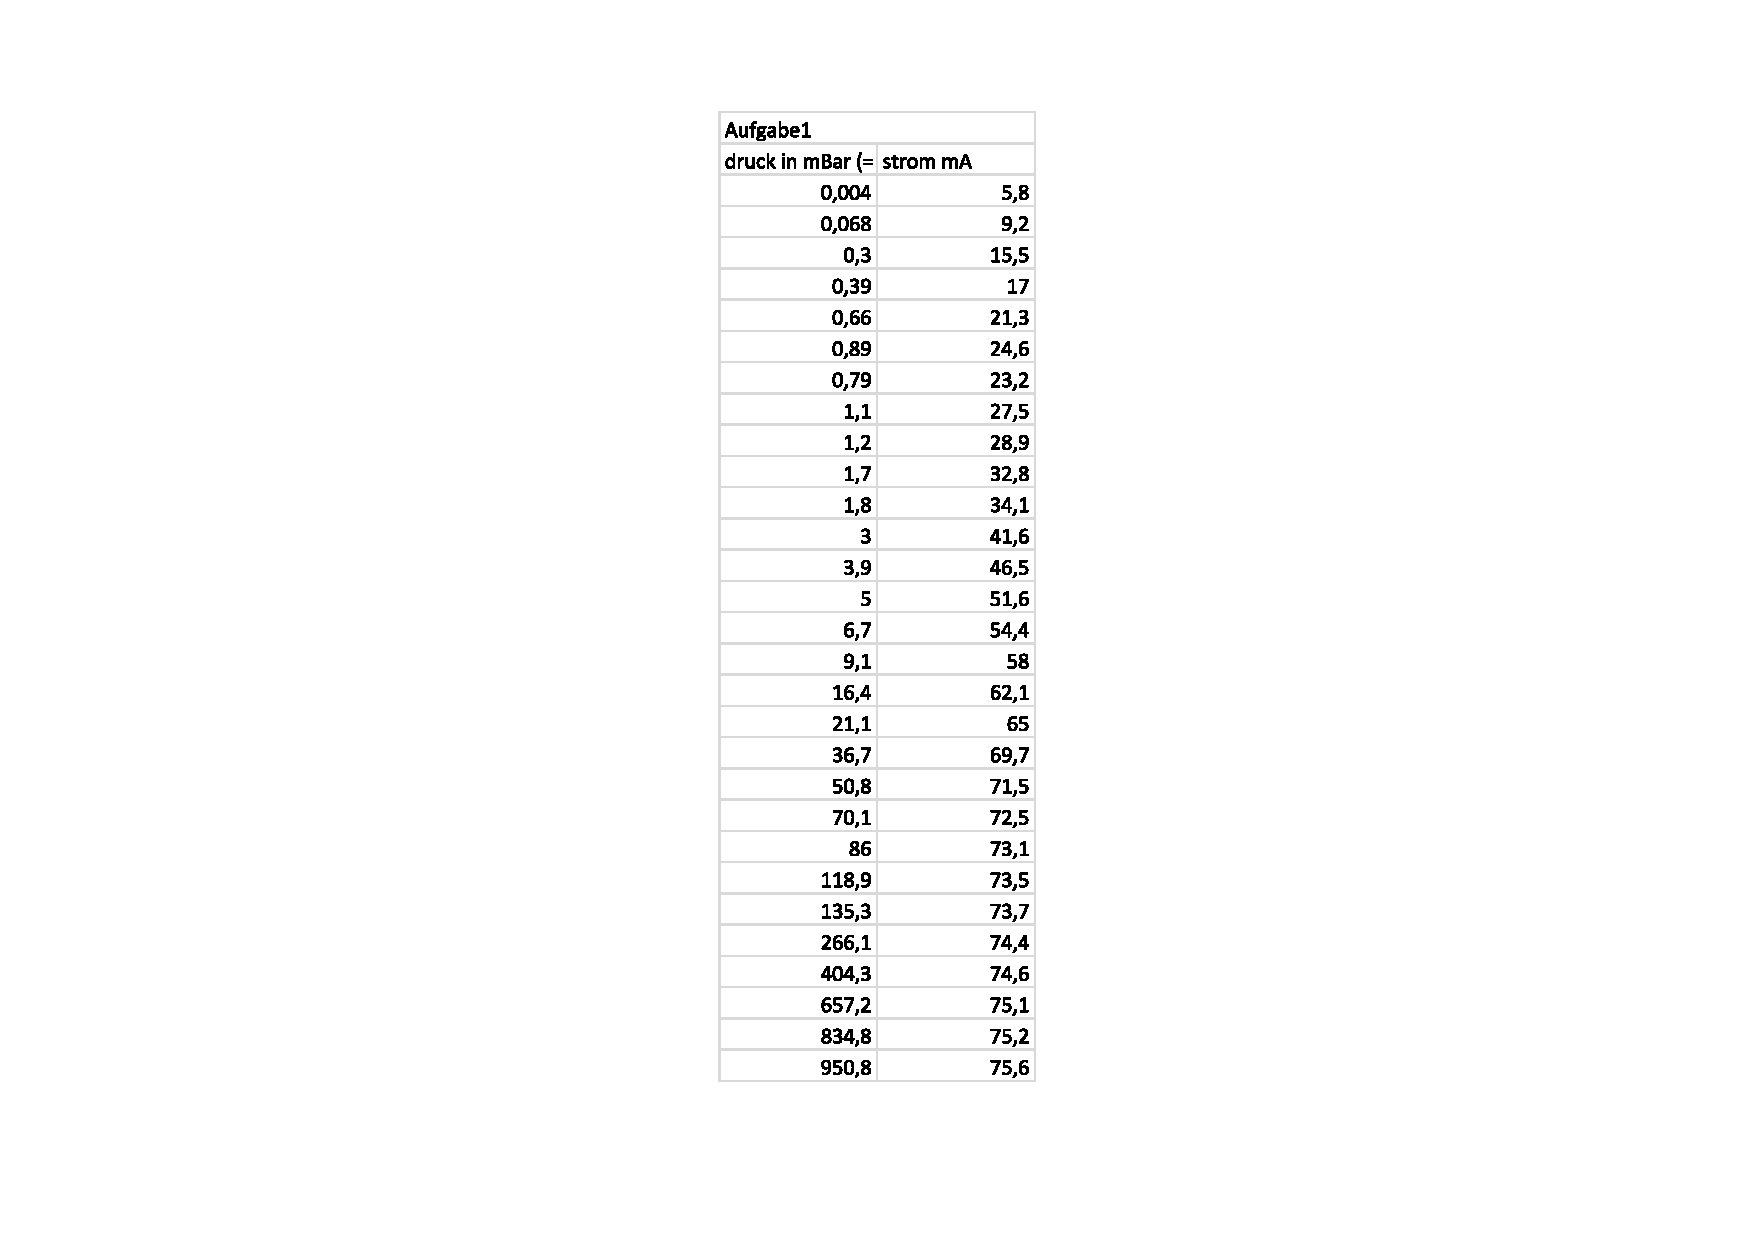
\includepdf[pages=-]{Aufgabe1Daten.pdf}
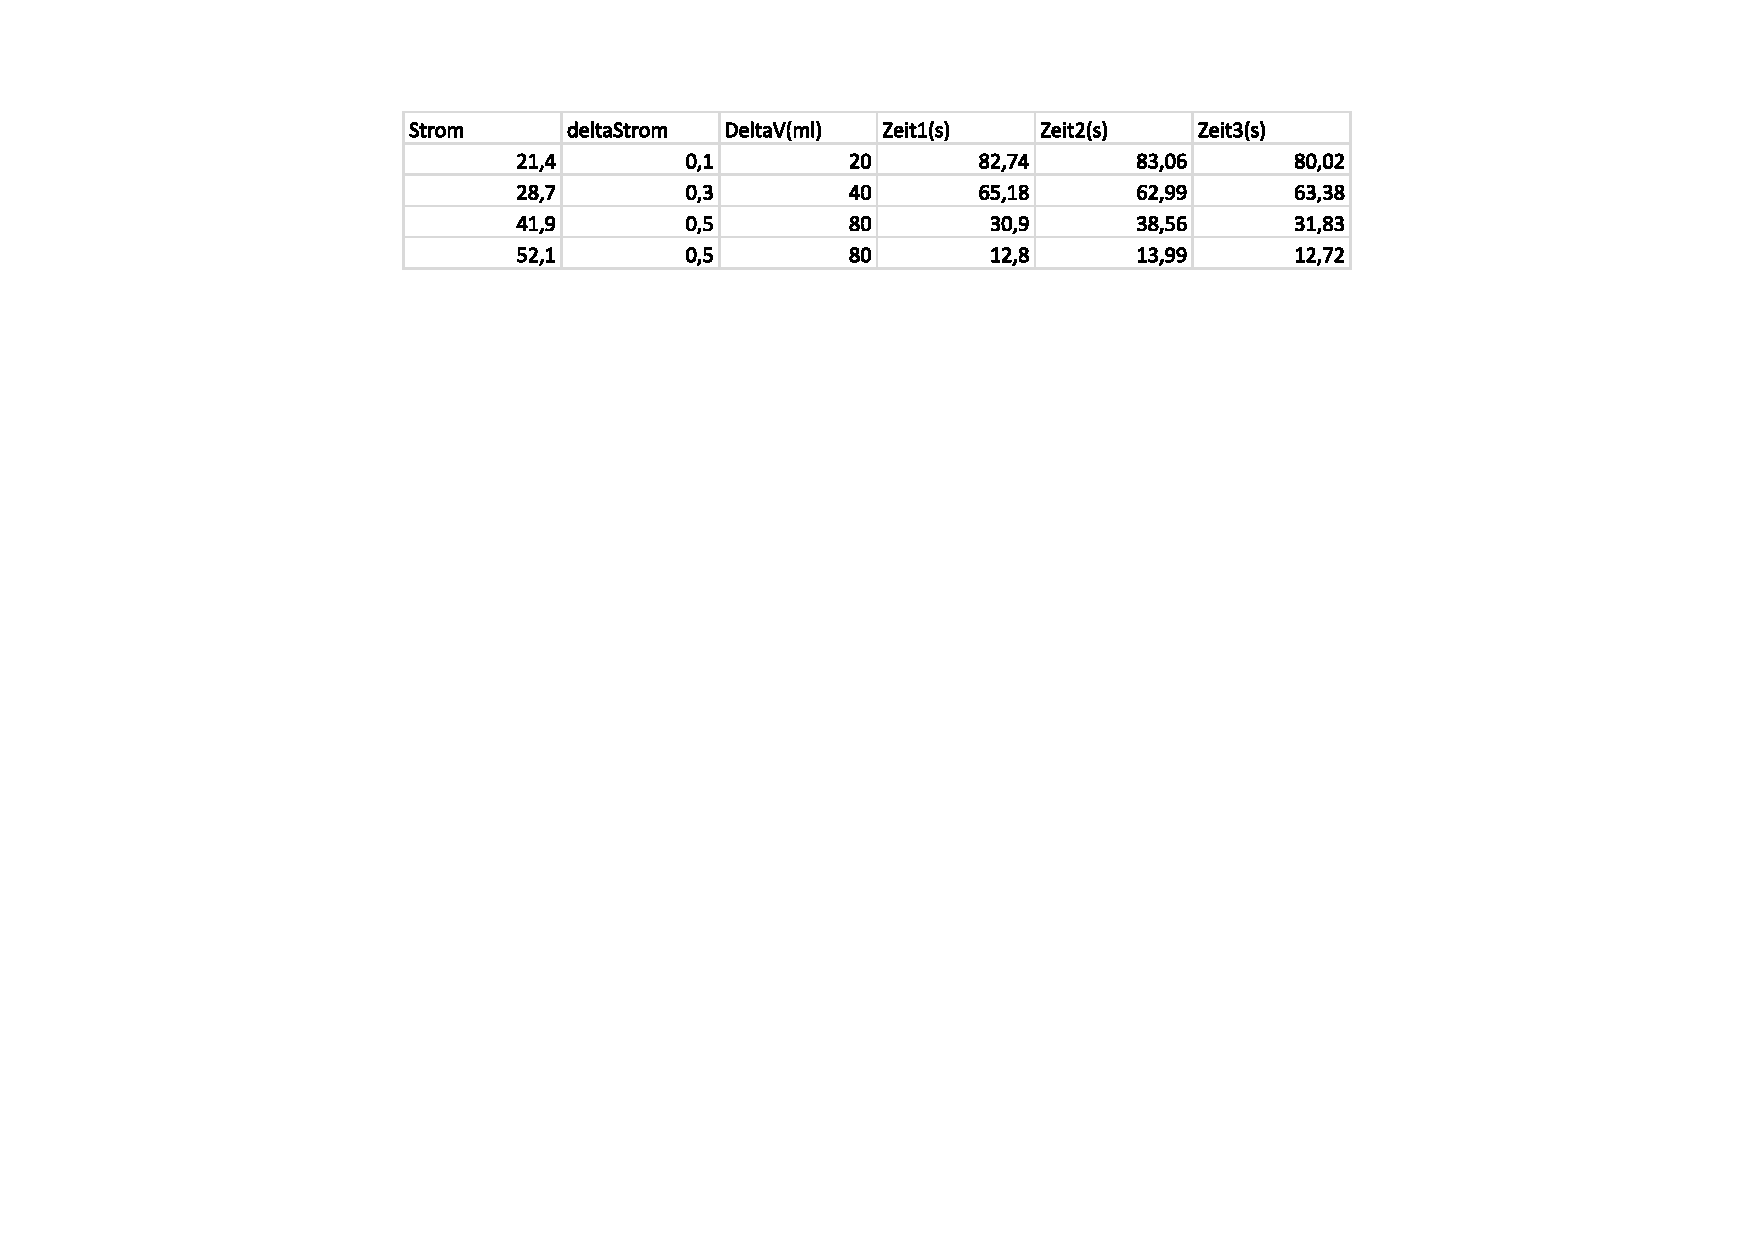
\includepdf[pages=-]{Aufgabe2Daten.pdf}
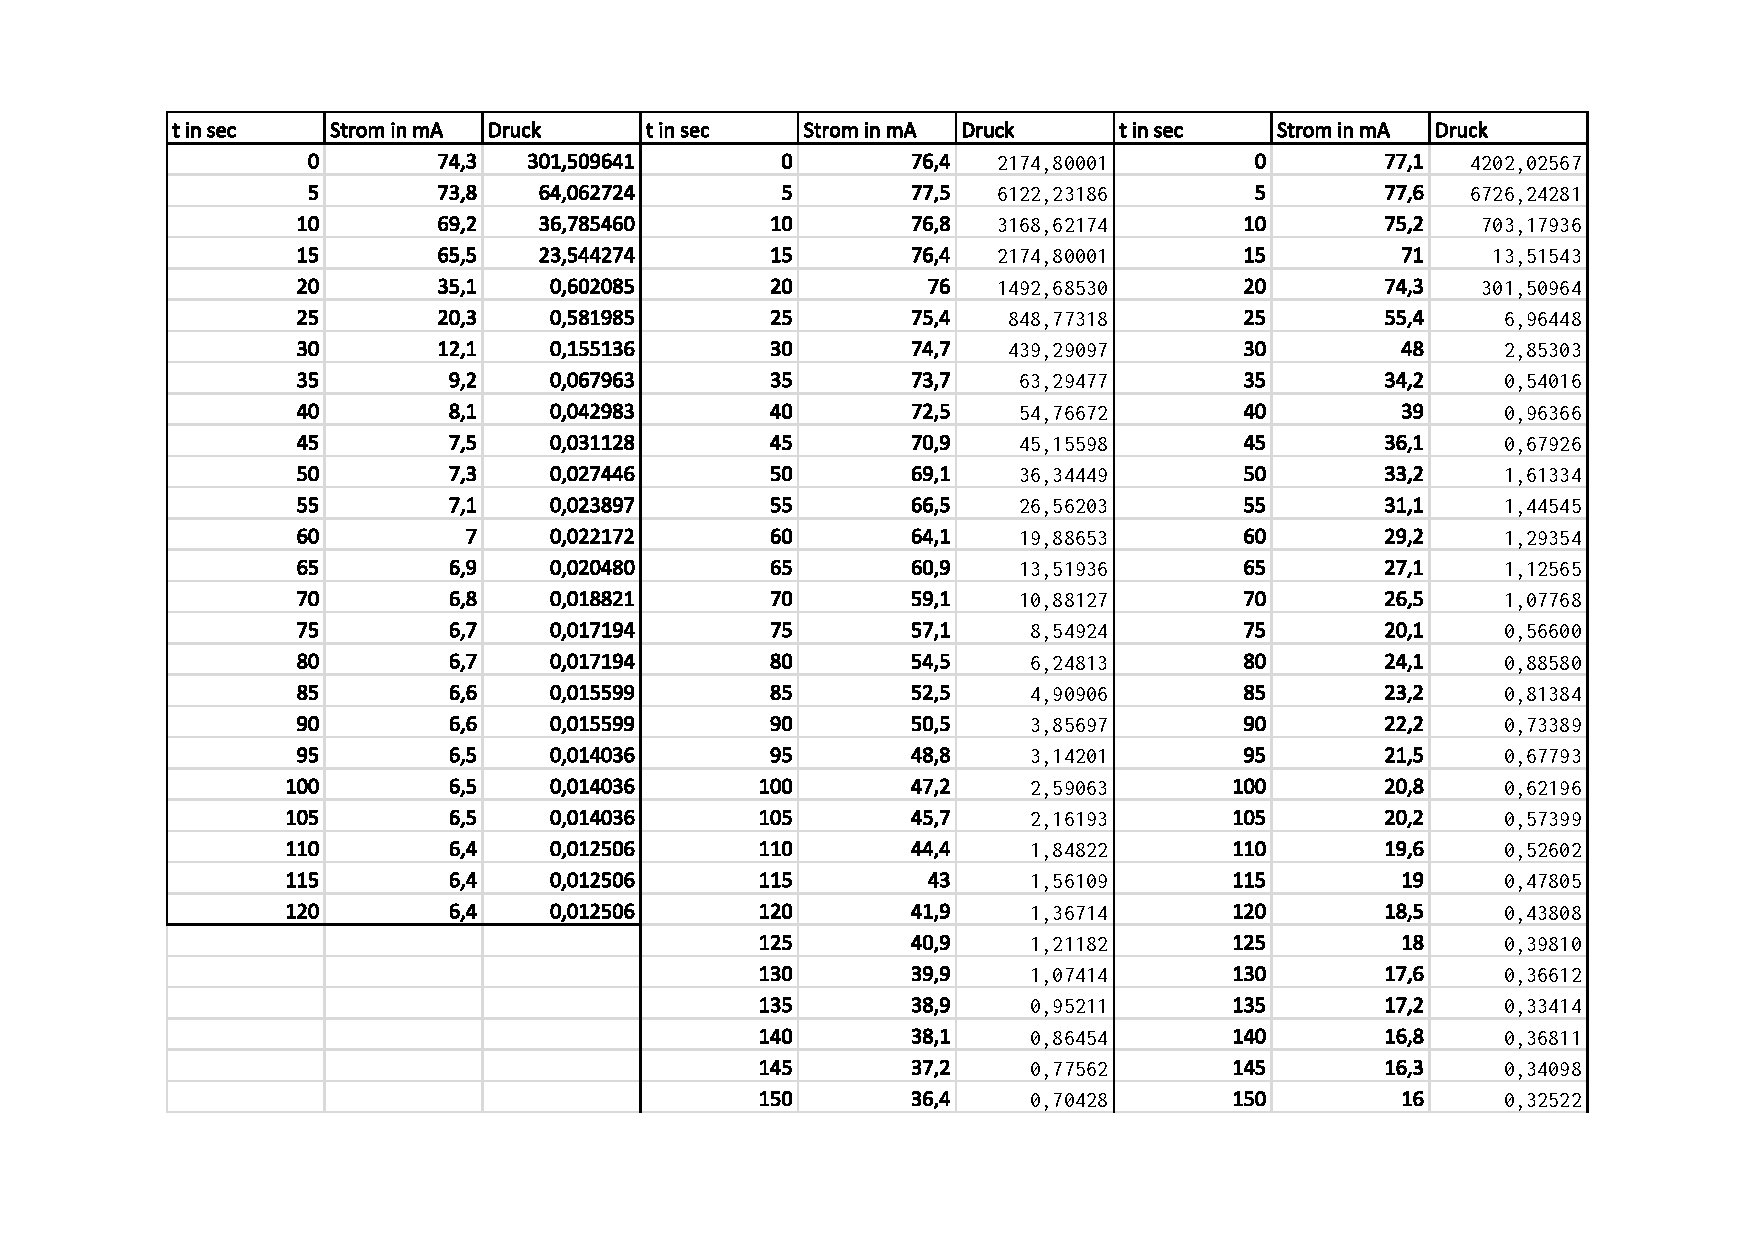
\includepdf[pages=-]{Aufgabe3Daten.pdf}
	
	
\end{document}